%\documentclass[11pt]{book}
%\usepackage{palatino}
%\usepackage{amsfonts,amsmath,amssymb}
%% \usepackage{graphicx}
%
%
%\ifx\pdftexversion\undefined
%    \usepackage[dvips]{graphicx}
%\else
%    \usepackage[pdftex]{graphicx}
%    \usepackage{epstopdf}
%    \epstopdfsetup{suffix=}
%\fi
%
%
%\begin{document}

%%%%%%%%%%%%%%%%%%%%%%%%%%%%%%%%%%%%%%%%
% Problem Set 4
%%%%%%%%%%%%%%%%%%%%%%%%%%%%%%%%%%%%%%%%

%\pagestyle{empty}
%{\noindent\bf Spring 2021 \hfill Firstname M.~Lastname}
%\vskip 16pt
%\centerline{\bf University of Central Florida}
%\centerline{\bf College of Business}
%\vskip 16pt
%\centerline{\bf QMB 6911}
%\centerline{\bf Capstone Project in Business Analytics}
%\vskip 10pt
%\centerline{\bf Solutions:  Problem Set \#4}
%\vskip 32pt
%\noindent

\section{Introduction}

This note summarizes the findings in the script
\texttt{Tractor\_Price\_Density.R},
which analyzes the prices of fly reels,
the dependent variable in the \texttt{TRACTOR7.csv} dataset.
The output includes plots of the histogram
and kernel-smoothed densities,
using a selection of tuning parameters.

\vfill
\pagebreak
\section{Relative Histogram of Fly Reel Prices}


First plot a histogram with the default options.

\begin{verbatim}
hist(tractor_sales[, 'saleprice'],
     main = 'Relative Histogram of Tractor Prices',
     xlab = 'Price',
     probability = TRUE)
\end{verbatim}


Figure \ref{fig:hist_saleprice} is
a histogram of the tractor prices
generated by the code block above.
%
\begin{figure}[h!]
  \centering
  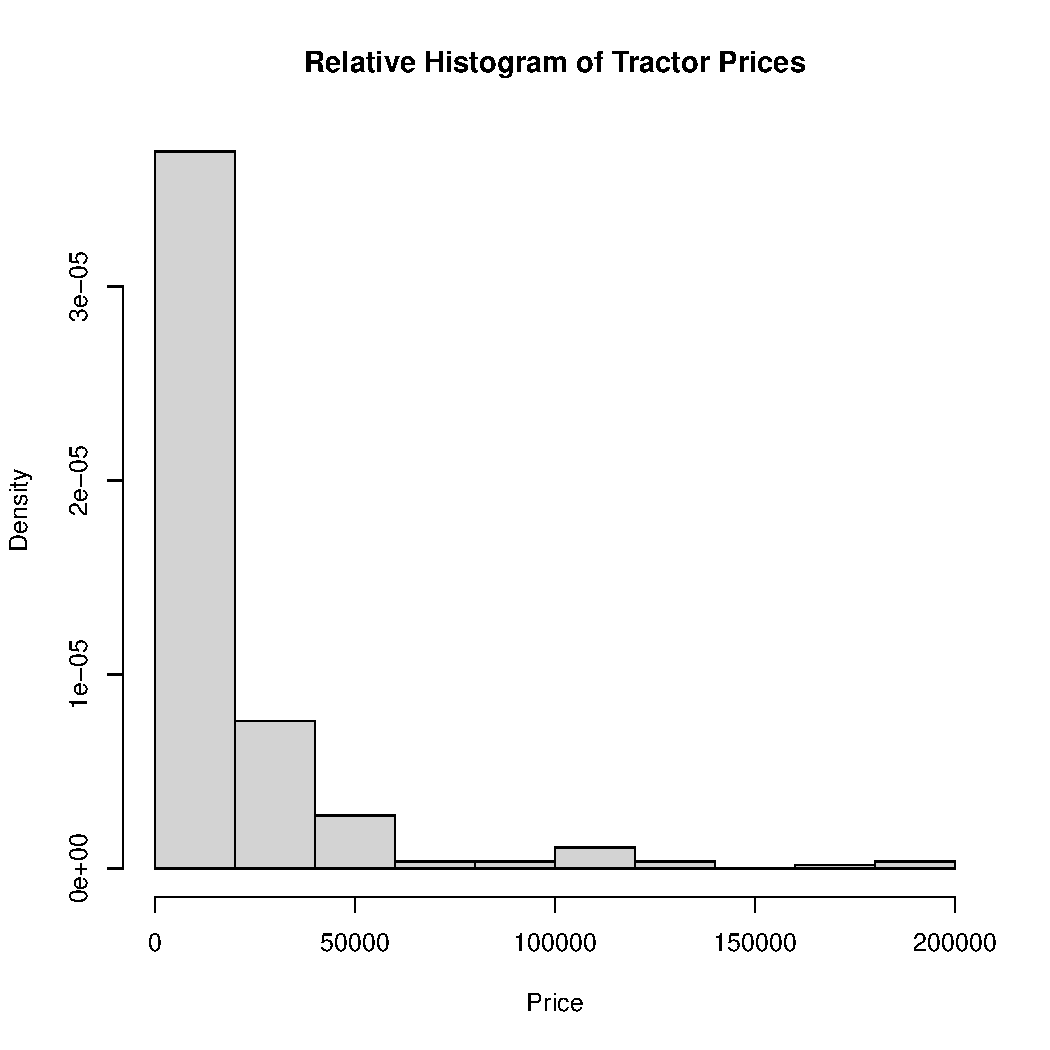
\includegraphics[scale = 0.5, keepaspectratio=true]{../Figures/hist_saleprice}
  \caption{Relative Histogram of Tractor Prices} \label{fig:hist_saleprice}
\end{figure}
%
%
Notice that there are some very large values.
Consider taking logs to bring outliers closer to the others.

\begin{verbatim}
# Generate a new variable log_saleprice.
tractor_sales[, 'log_saleprice'] <- log(tractor_sales[, 'saleprice'])
\end{verbatim}

Now plot the histogram for log of saleprice,
depicted in Figure \ref{fig:hist_log_saleprice}.

\begin{verbatim}
hist(tractor_sales[, 'log_saleprice'],
     main = 'Histogram of the Logarithm of Tractor Prices',
     xlab = 'Logarithm of Price',
     probability = TRUE)
\end{verbatim}


\begin{figure}[h!]
  \centering
  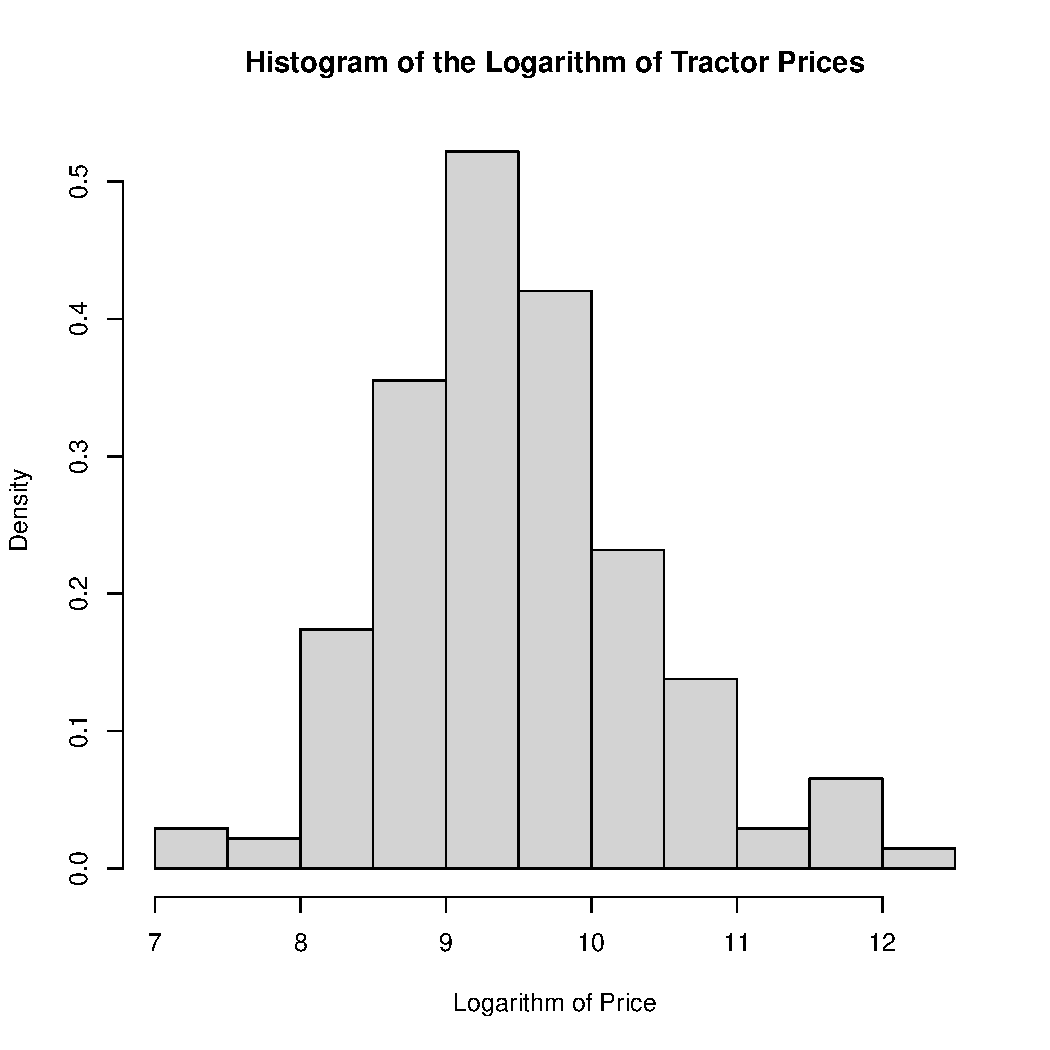
\includegraphics[scale = 0.5, keepaspectratio=true]{../Figures/hist_log_saleprice}
  \caption{Relative Histogram of the Logarithm of Tractor Prices} \label{fig:hist_log_saleprice}
\end{figure}

With this transformation, the variable appears much better behaved.
It looks almost normally distributed.

Now we will consider adjusting the tuning parameter for the number of
bars in the chart for the histogram.
%
A low number of breaks may give a smoother plot but
it may not be very informative, as in Figure \ref{fig:hist_log_saleprice_br5}.

\begin{verbatim}
hist(tractor_sales[, 'log_saleprice'], breaks = 5,
     main = c('Histogram of the Logarithm of Tractor Prices',
              'Number of Breaks: 5'),
     xlab = 'Logarithm of Price',
     probability = TRUE)
\end{verbatim}


\begin{figure}[h!]
  \centering
  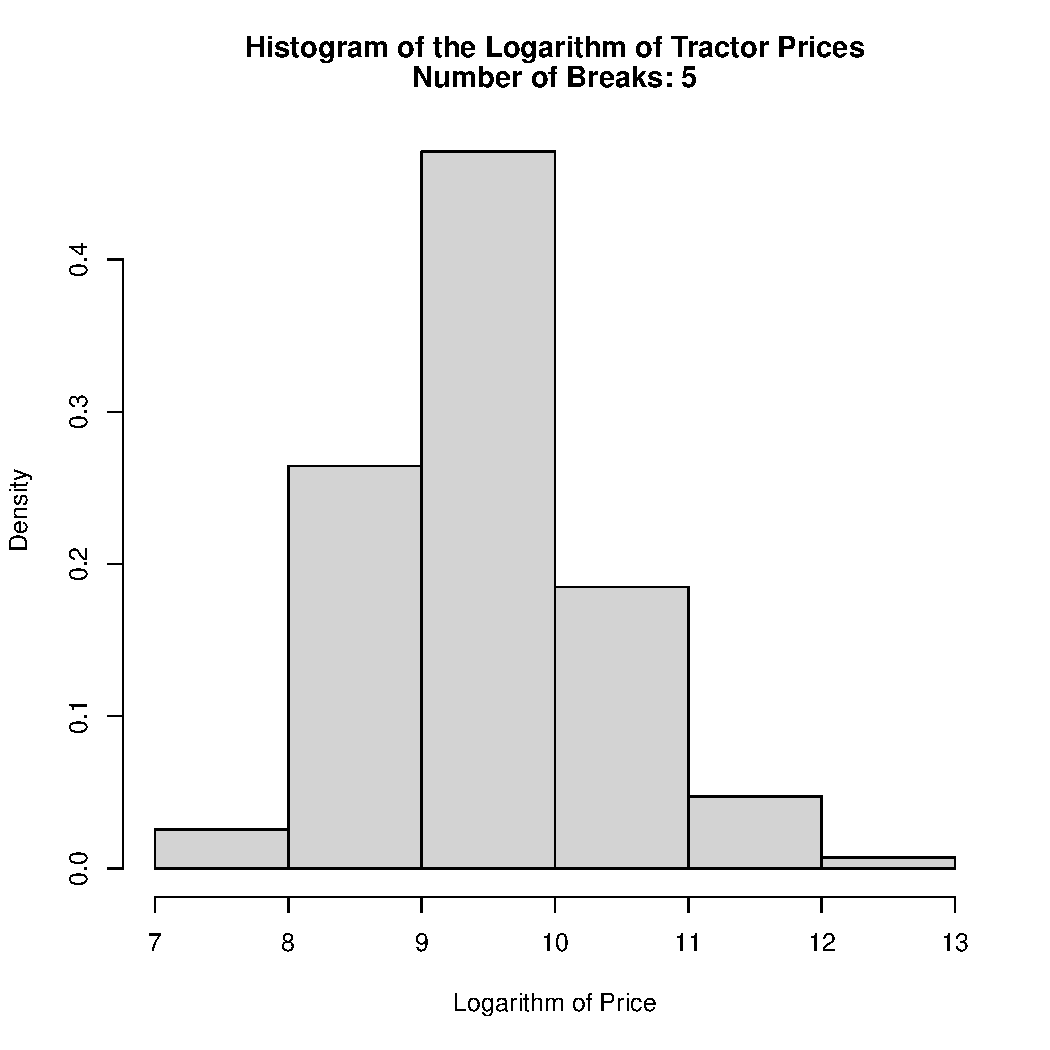
\includegraphics[scale = 0.5, keepaspectratio=true]{../Figures/hist_log_saleprice_br5}
  \caption{Relative Histogram of the Logarithm of Tractor Prices (Breaks: $5$)} \label{fig:hist_log_saleprice_br5}
\end{figure}

On the other extreme,
a high number of breaks gives a sparsely populated
and jagged plot.
Figure \ref{fig:hist_log_saleprice_br50}
shows such an example.

\begin{verbatim}
hist(tractor_sales[, 'log_saleprice'], breaks = 50,
     main = c('Histogram of the Logarithm of Tractor Prices',
              'Number of Breaks: 5'),
     xlab = 'Logarithm of Price',
     probability = TRUE)
\end{verbatim}

\begin{figure}[h!]
  \centering
  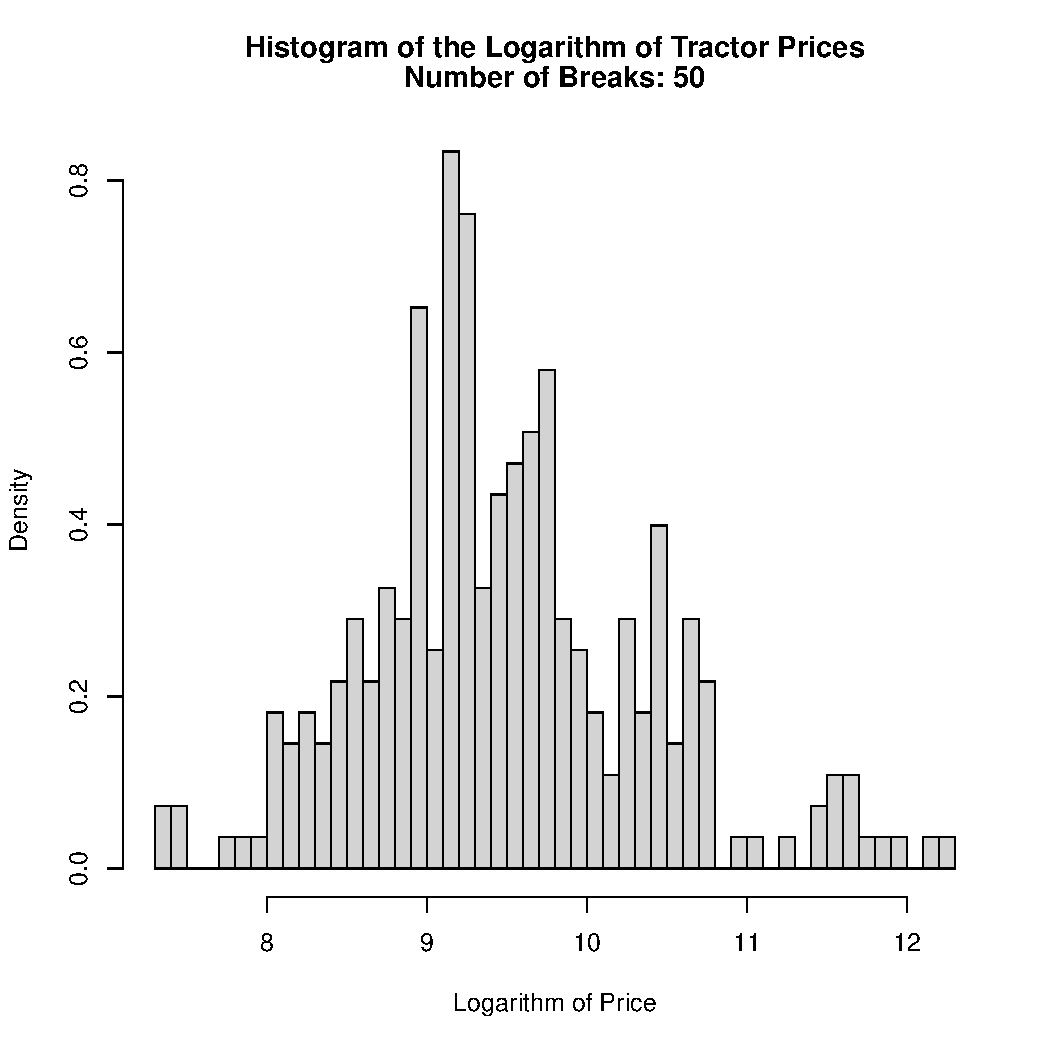
\includegraphics[scale = 0.5, keepaspectratio=true]{../Figures/hist_log_saleprice_br50}
  \caption{Relative Histogram of the Logarithm of Tractor Prices (Breaks: $50$)} \label{fig:hist_log_saleprice_br50}
\end{figure}

\pagebreak
In the limit, the bars can be very small
to the point that each bar is a pixel wide:
approximating a continuous function.
To smooth it out, the nonparametric technique of
kernel smoothing with produce a continuous function.


\pagebreak
\section{Probability Density Function of Tractor Prices}

Kernel-density smoothing is an example of a nonparametric method,
that is, a model without parameters,
such as the slope coefficients $\beta$ in a regression model.
You may have used nonparametric methods to plot a density.
In fact, we have just used a rudimentary form of nonparanetric method
when we plotted the histograms above.


Figure \ref{fig:density_saleprice} depicts
the kernel-smoothed probability density function of the natural logarithm of
price.
\begin{verbatim}
price_density <- density(tractor_sales[, 'saleprice'])
plot(price_density,
     main = 'Kernel-Smoothed Density of Tractor Prices',
     xlab = 'Price')
\end{verbatim}


\begin{figure}[h!]
  \centering
  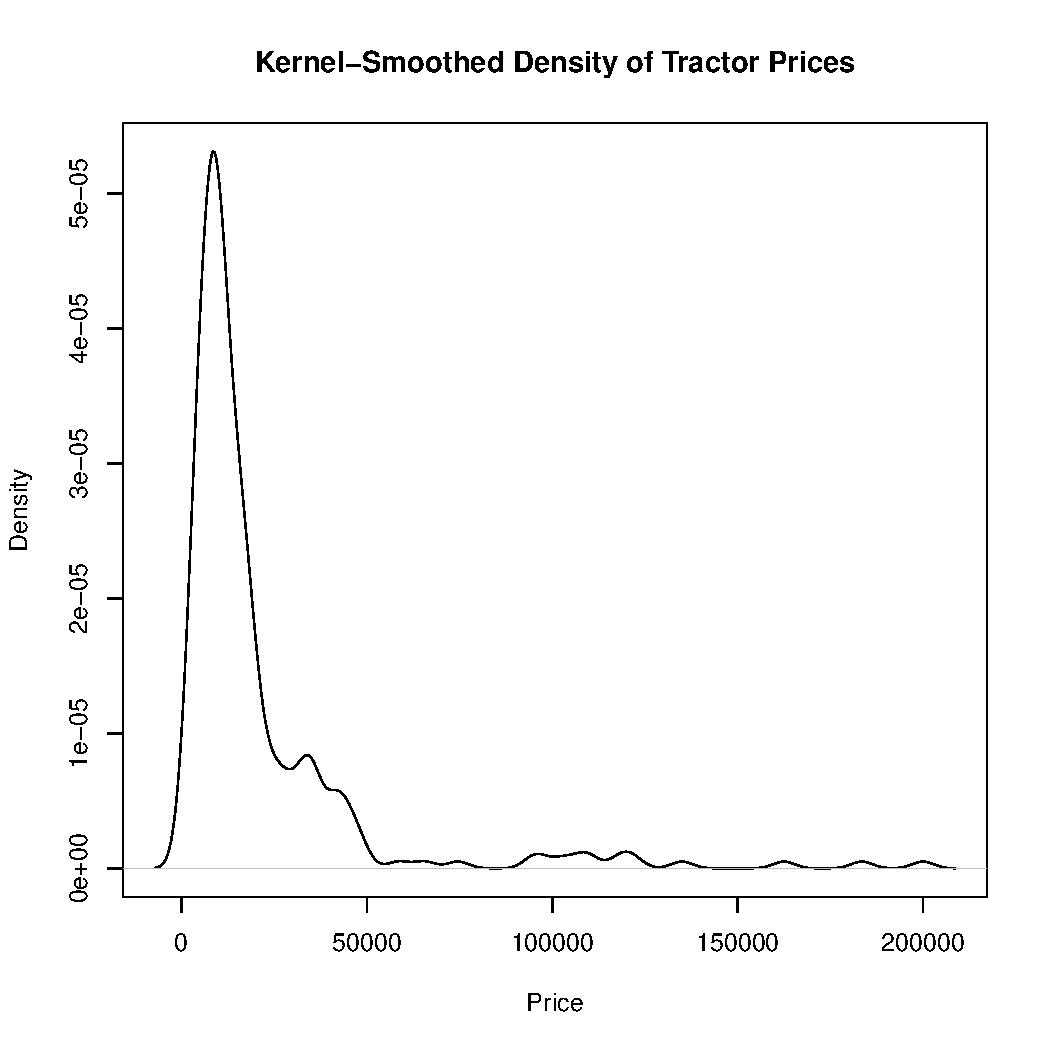
\includegraphics[scale = 0.5, keepaspectratio=true]{../Figures/density_saleprice}
  \caption{Probability Density Function of Tractor Prices} \label{fig:density_saleprice}
\end{figure}

\pagebreak
In the default, the bandwidth is chosen using an algorithm.
See the help for density.

\begin{verbatim}
> attributes(price_density)
$names
[1] "x"         "y"         "bw"        "n"
[5] "call"      "data.name" "has.na"

$class
[1] "density"

> price_density$bw
[1] 2875.455
>
\end{verbatim}

The default algorithm for this variable sets the bandwidth to \$$2,875$.
You can choose the bandwidth as a tuning parameter.
Try a larger value as in the following code block.

\begin{verbatim}
price_density <- density(tractor_sales[, 'saleprice'],
                         bw = 10000)
plot(price_density,
     main = c('Kernel-Smoothed Density of Tractor Prices',
              'Bandwidth: 10,000'),
     xlab = 'Price')
\end{verbatim}

Figure \ref{fig:density_saleprice_bw10000} depicts
the kernel-smoothed probability density function
with a bandwidth of $10,000$.


\begin{figure}[h!]
  \centering
  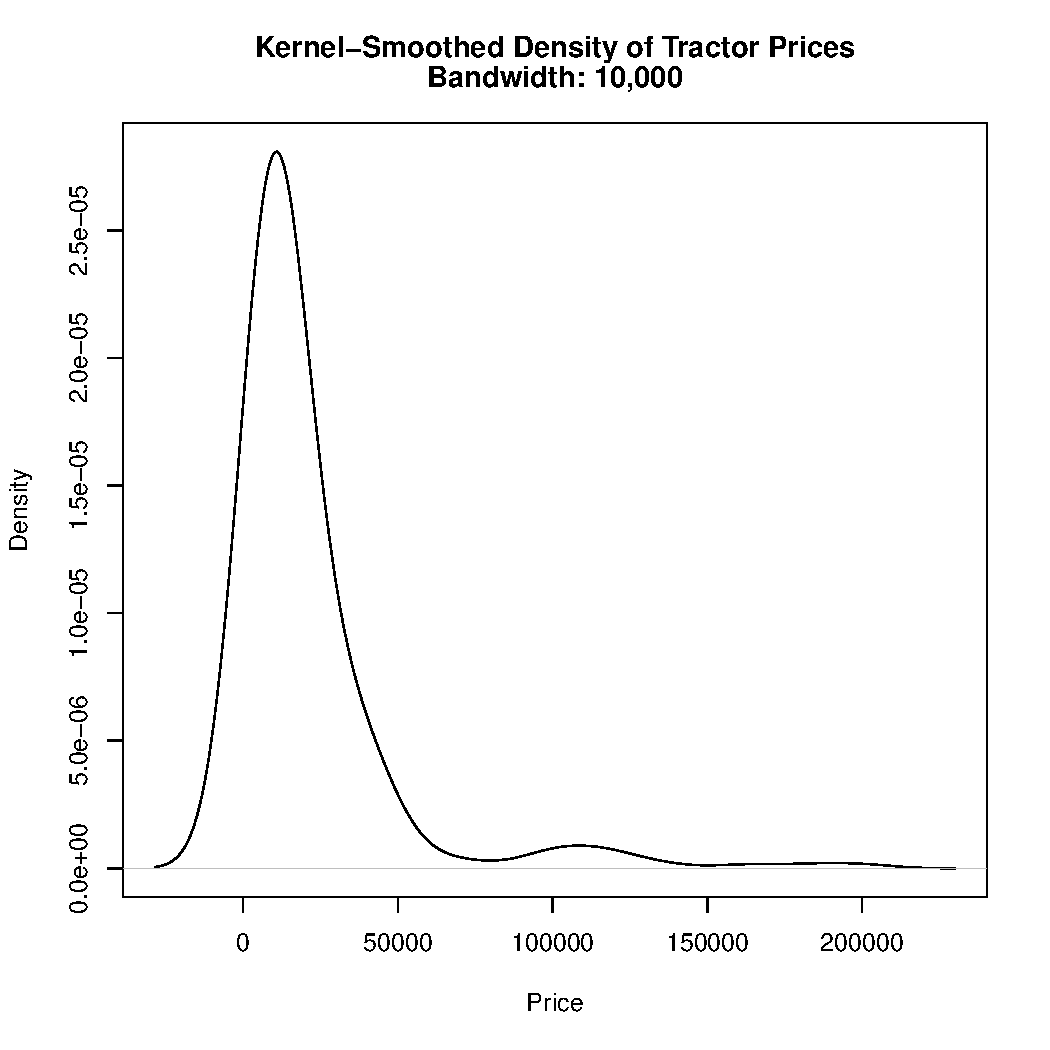
\includegraphics[scale = 0.5, keepaspectratio=true]{../Figures/density_saleprice_bw10000}
  \caption{Probability Density Function of Tractor Prices (Bandwidth: $10,000$)} \label{fig:density_saleprice_bw10000}
\end{figure}

\pagebreak
A bigger bandwidth gives you a smooth density,
but might smooth over the details.
A smaller bandwidth might make the density too noisy.


\begin{verbatim}
price_density <- density(tractor_sales[, 'saleprice'],
                         bw = 1000)
plot(price_density,
     main = c('Kernel-Smoothed Density of Tractor Prices',
              'Bandwidth: 1,000'),
     xlab = 'Price')
\end{verbatim}


\begin{figure}[h!]
  \centering
  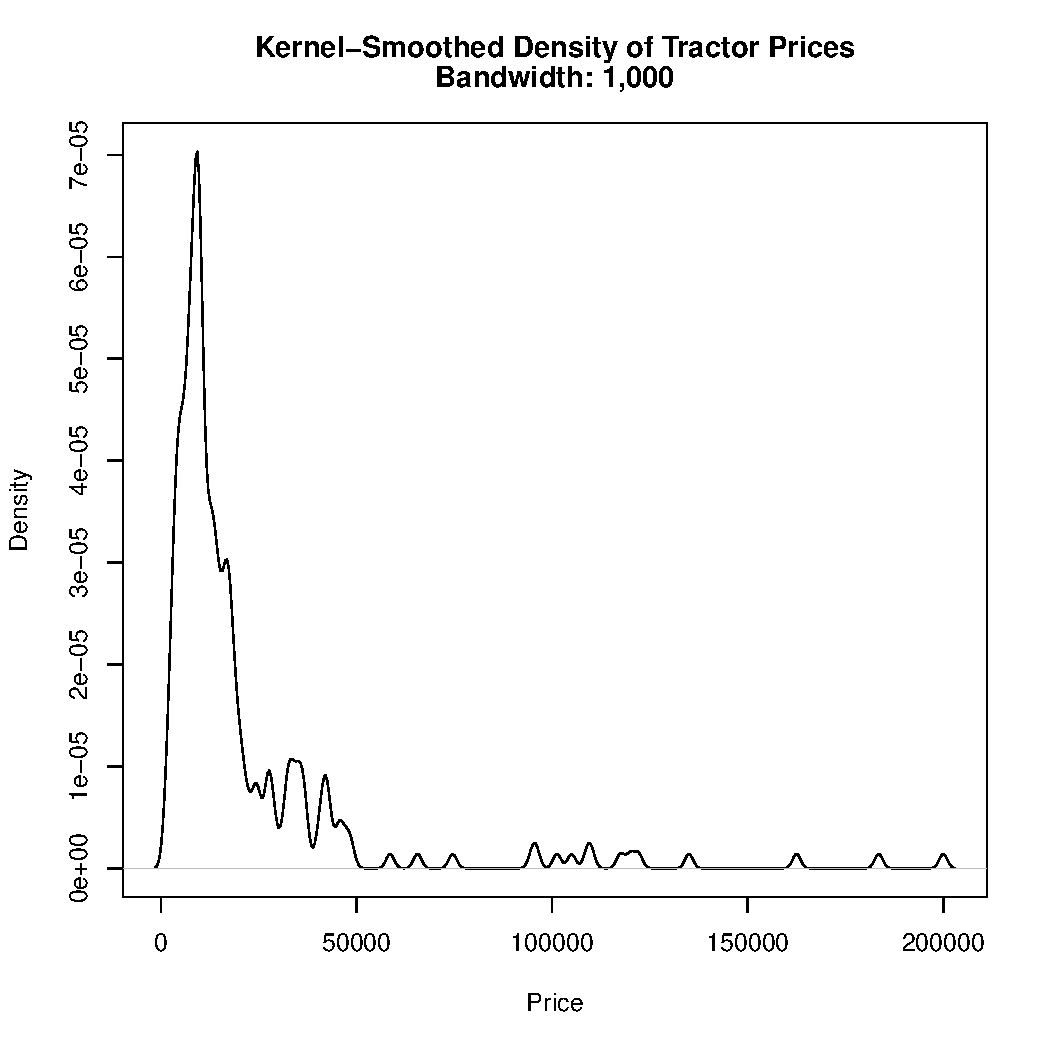
\includegraphics[scale = 0.5, keepaspectratio=true]{../Figures/density_saleprice_bw1000}
  \caption{Probability Density Function of Tractor Prices (Bandwidth: $10,00$)} \label{fig:density_saleprice_bw1000}
\end{figure}

In Figure \ref{fig:density_saleprice_bw1000},
we see many jagged changes that are more closely related
with the particular values observed
than with the population density.

\pagebreak
We can do something similar to predict one variable
with the others.
Before that, we will transform the dependent variable,
after analyzing it in greater detail in future problem sets.
For now, we can plot the logarithm of the dependent variable,
with a bandwidth of $0.20$, which is appropriate for the price levels on a log scale..


\begin{verbatim}
log_price_density <- density(tractor_sales[, 'log_saleprice'],
                         bw = 0.20)
plot(log_price_density,
     main = c('Density of the Logarithm of Tractor Prices',
              'Bandwidth: 0.20'),
     xlab = 'Logarithm of Price')
\end{verbatim}

\begin{figure}[h!]
  \centering
  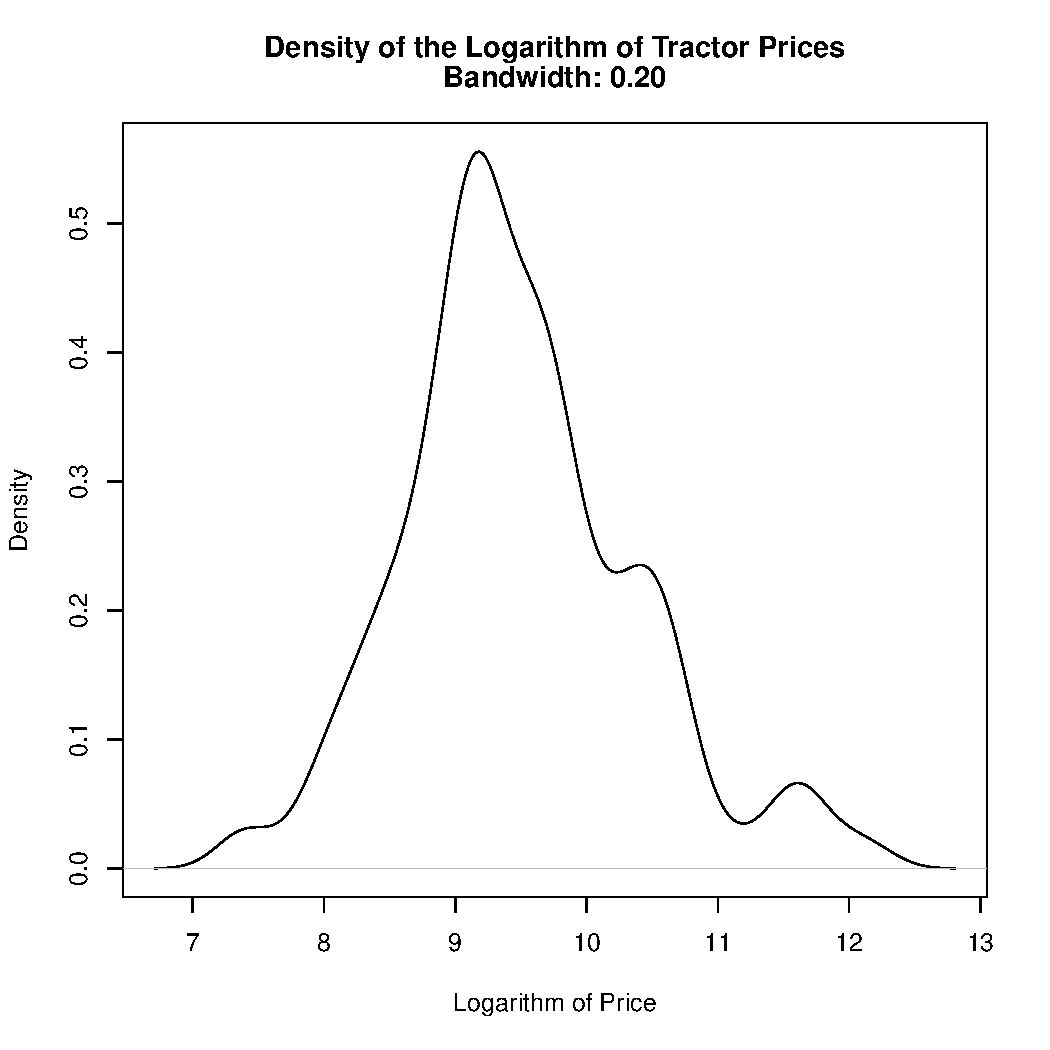
\includegraphics[scale = 0.5, keepaspectratio=true]{../Figures/density_log_saleprice_bw020}
  \caption{Probability Density Function of the Logarithm of Tractor Prices (Bandwidth: $0.20$)} \label{fig:density_log_saleprice_bw020}
\end{figure}


The density plot
shown in Figure \ref{fig:density_log_saleprice_bw020}
is much better behaved and is a good starting point to
analyze the data in a regression model.



%%%%%%%%%%%%%%%%%%%%%%%%%%%%%%%%%%%%%%%%
% \end{document}
%%%%%%%%%%%%%%%%%%%%%%%%%%%%%%%%%%%%%%%%
